\documentclass[11pt]{article}
\usepackage[textwidth=18.0cm, textheight=23.0cm, top=2.0cm]{geometry}
\usepackage{pst-all}
\usepackage{amssymb}
\usepackage{tikz}
\usepackage{underscore}\begin{document}
\pagestyle{empty}


ClassName: \underline{\textbf{Class_03.2bp-2}}
\par
BinSize: \underline{\textbf{40 × 40}}
\par
ReduceSize: \underline{\textbf{40 × 40}}
\par
TypeNum: \underline{\textbf{20}}
\par
Num: \underline{\textbf{20}}
\par
OutS: \underline{\textbf{9600}}
\par
InS: \underline{\textbf{7055}}
\par
Rate: \underline{\textbf{0.735}}
\par
UB: \underline{\textbf{6}}
\par
LB0: \underline{\textbf{5}}
\par
LB: \underline{\textbf{6}}
\par
LBWithCut: \underline{\textbf{6}}
\par
NodeCut: \underline{\textbf{0}}
\par
ExtendedNodeCnt: \underline{\textbf{1}}
\par
GenNodeCnt: \underline{\textbf{1}}
\par
PrimalNode: \underline{\textbf{0}}
\par
ColumnCount: \underline{\textbf{55}}
\par
TotalCutCount: \underline{\textbf{0}}
\par
RootCutCount: \underline{\textbf{0}}
\par
LPSolverCnt: \underline{\textbf{50}}
\par
PricingSolverCnt: \underline{\textbf{50}}
\par
BranchAndBoundNum: \underline{\textbf{1}}
\par
isOpt: \underline{\textbf{true}}
\par
TimeOnInitSolution: \underline{\textbf{600.000 s}}
\par
TimeOnPrimal: \underline{\textbf{0.000 s}}
\par
TimeOnPricing: \underline{\textbf{1.596 s}}
\par
TimeOnRmp: \underline{\textbf{0.091 s}}
\par
TotalTime: \underline{\textbf{601.984 s}}
\par
\newpage


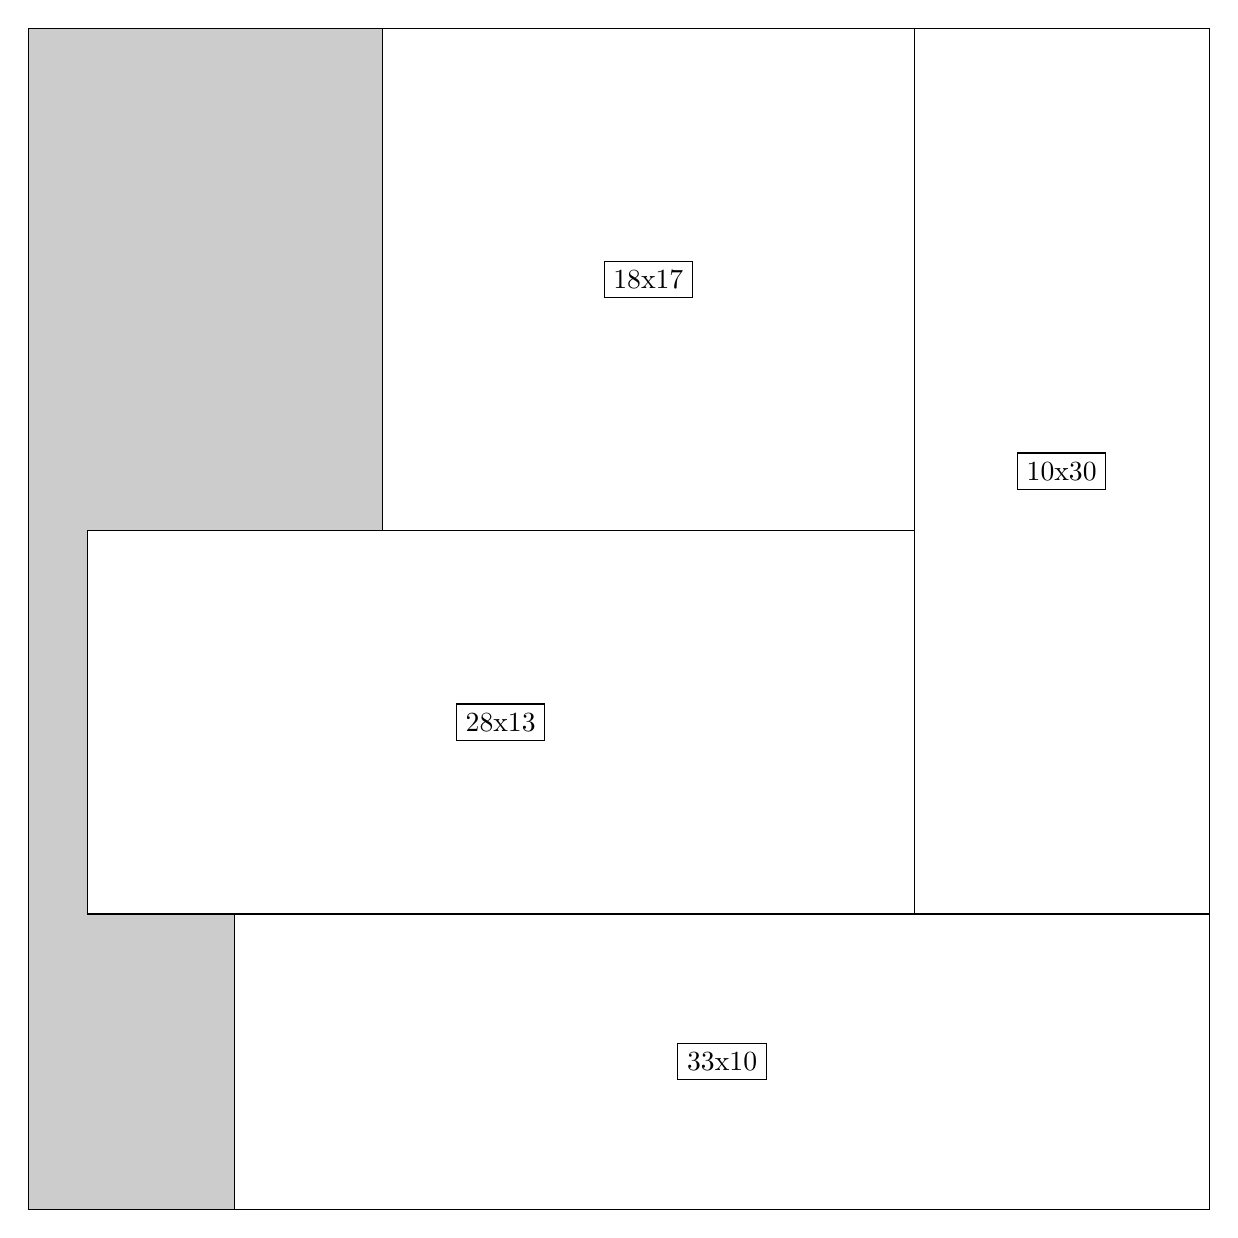
\begin{tikzpicture}[shorten >=1pt,scale=1.0,every node/.style={scale=1.0},->]
\tikzstyle{vertex}=[circle,fill=black!25,minimum size=14pt,inner sep=0pt]
\filldraw[fill=gray!40!white, draw=black] (0,0) rectangle (15.0,15.0);
\foreach \name/\x/\y/\w/\h in {33x10/2.625/0.0/12.375/3.75,10x30/11.25/3.75/3.75/11.25,28x13/0.75/3.75/10.5/4.875,18x17/4.5/8.625/6.75/6.375}
\filldraw[fill=white!40!white, draw=black] (\x,\y) rectangle node[draw] (\name) {\name} ++(\w,\h);
\end{tikzpicture}


w =33 , h =10 , x =7 , y =0 , v =330
\par
w =10 , h =30 , x =30 , y =10 , v =300
\par
w =28 , h =13 , x =2 , y =10 , v =364
\par
w =18 , h =17 , x =12 , y =23 , v =306
\par
\newpage


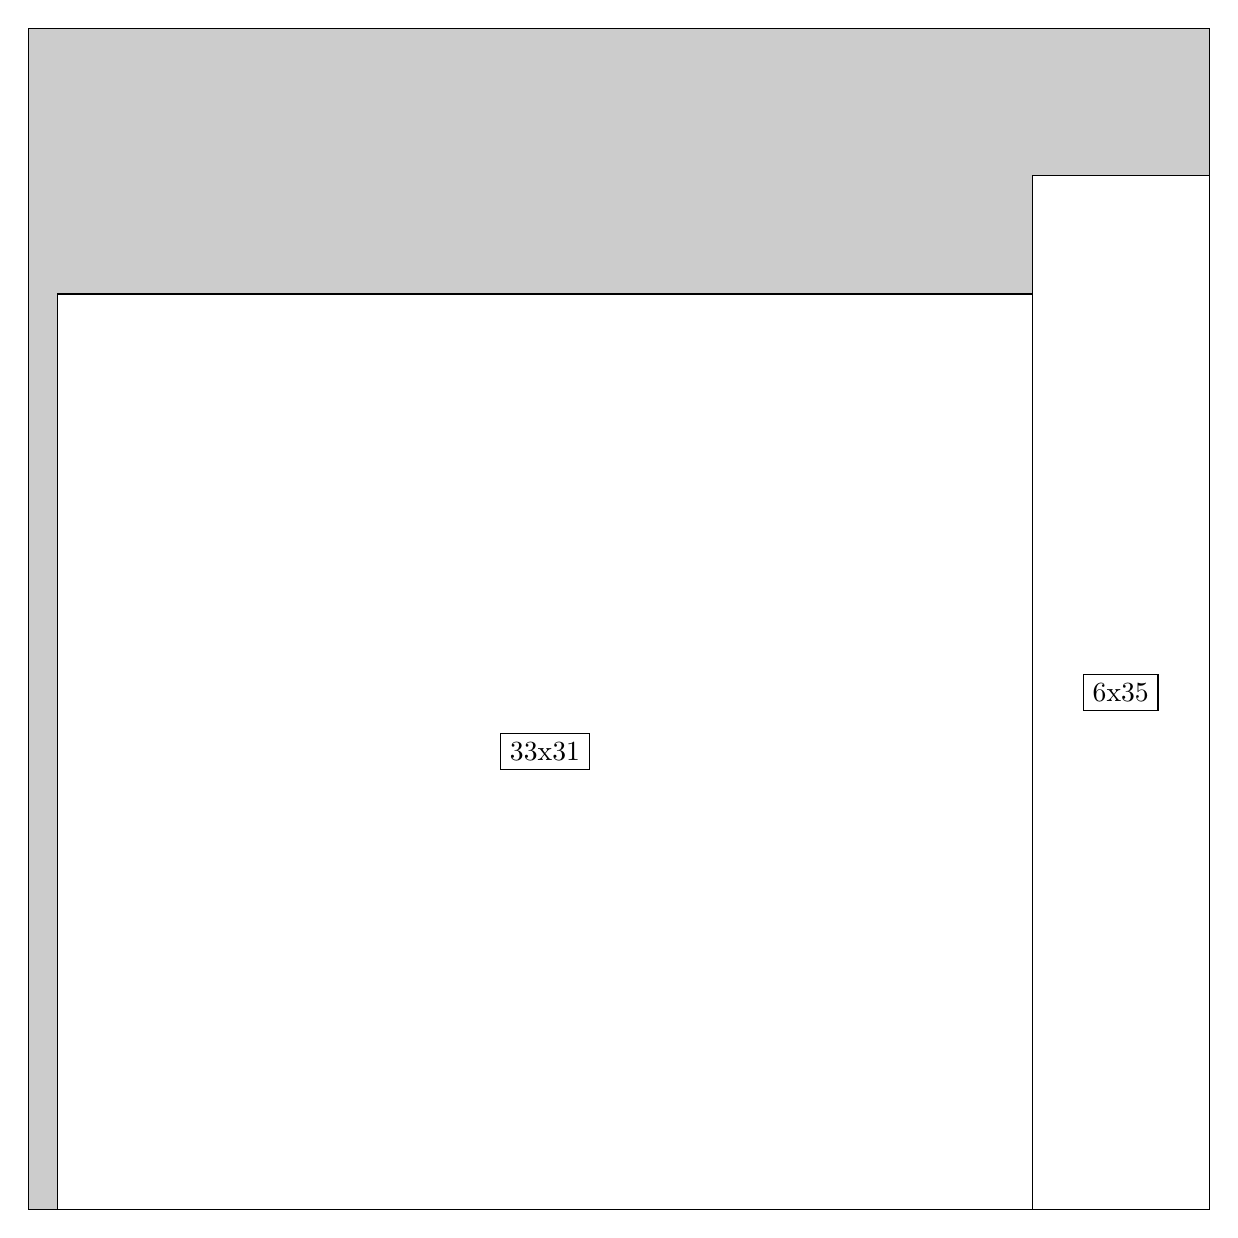
\begin{tikzpicture}[shorten >=1pt,scale=1.0,every node/.style={scale=1.0},->]
\tikzstyle{vertex}=[circle,fill=black!25,minimum size=14pt,inner sep=0pt]
\filldraw[fill=gray!40!white, draw=black] (0,0) rectangle (15.0,15.0);
\foreach \name/\x/\y/\w/\h in {6x35/12.75/0.0/2.25/13.125,33x31/0.375/0.0/12.375/11.625}
\filldraw[fill=white!40!white, draw=black] (\x,\y) rectangle node[draw] (\name) {\name} ++(\w,\h);
\end{tikzpicture}


w =6 , h =35 , x =34 , y =0 , v =210
\par
w =33 , h =31 , x =1 , y =0 , v =1023
\par
\newpage


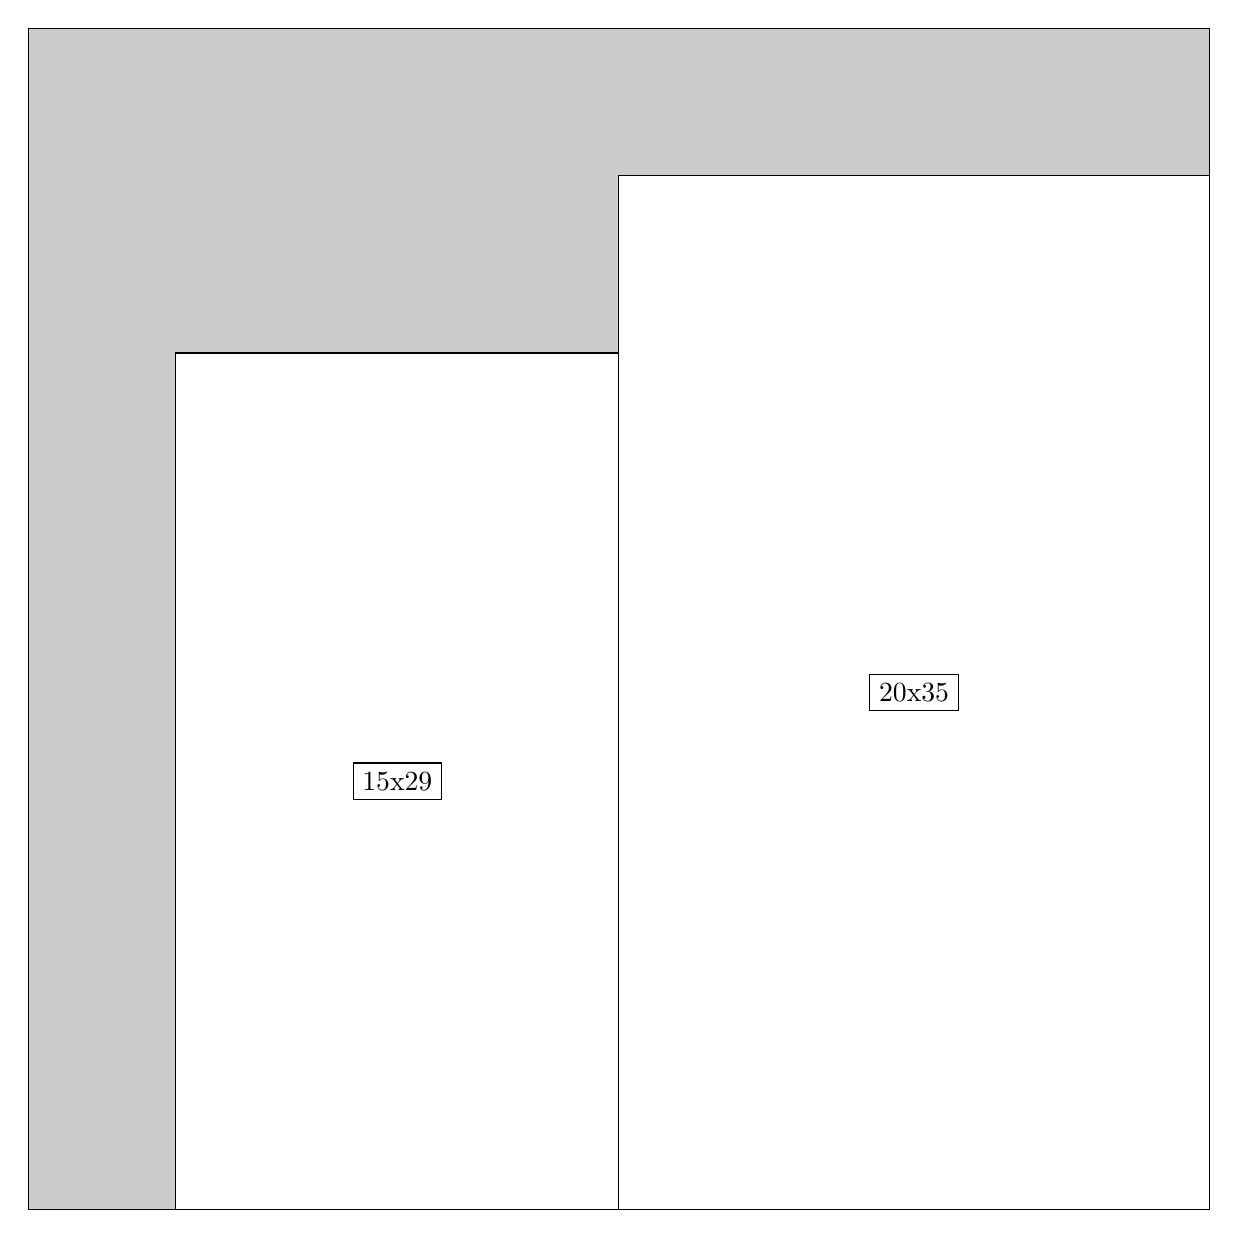
\begin{tikzpicture}[shorten >=1pt,scale=1.0,every node/.style={scale=1.0},->]
\tikzstyle{vertex}=[circle,fill=black!25,minimum size=14pt,inner sep=0pt]
\filldraw[fill=gray!40!white, draw=black] (0,0) rectangle (15.0,15.0);
\foreach \name/\x/\y/\w/\h in {20x35/7.5/0.0/7.5/13.125,15x29/1.875/0.0/5.625/10.875}
\filldraw[fill=white!40!white, draw=black] (\x,\y) rectangle node[draw] (\name) {\name} ++(\w,\h);
\end{tikzpicture}


w =20 , h =35 , x =20 , y =0 , v =700
\par
w =15 , h =29 , x =5 , y =0 , v =435
\par
\newpage


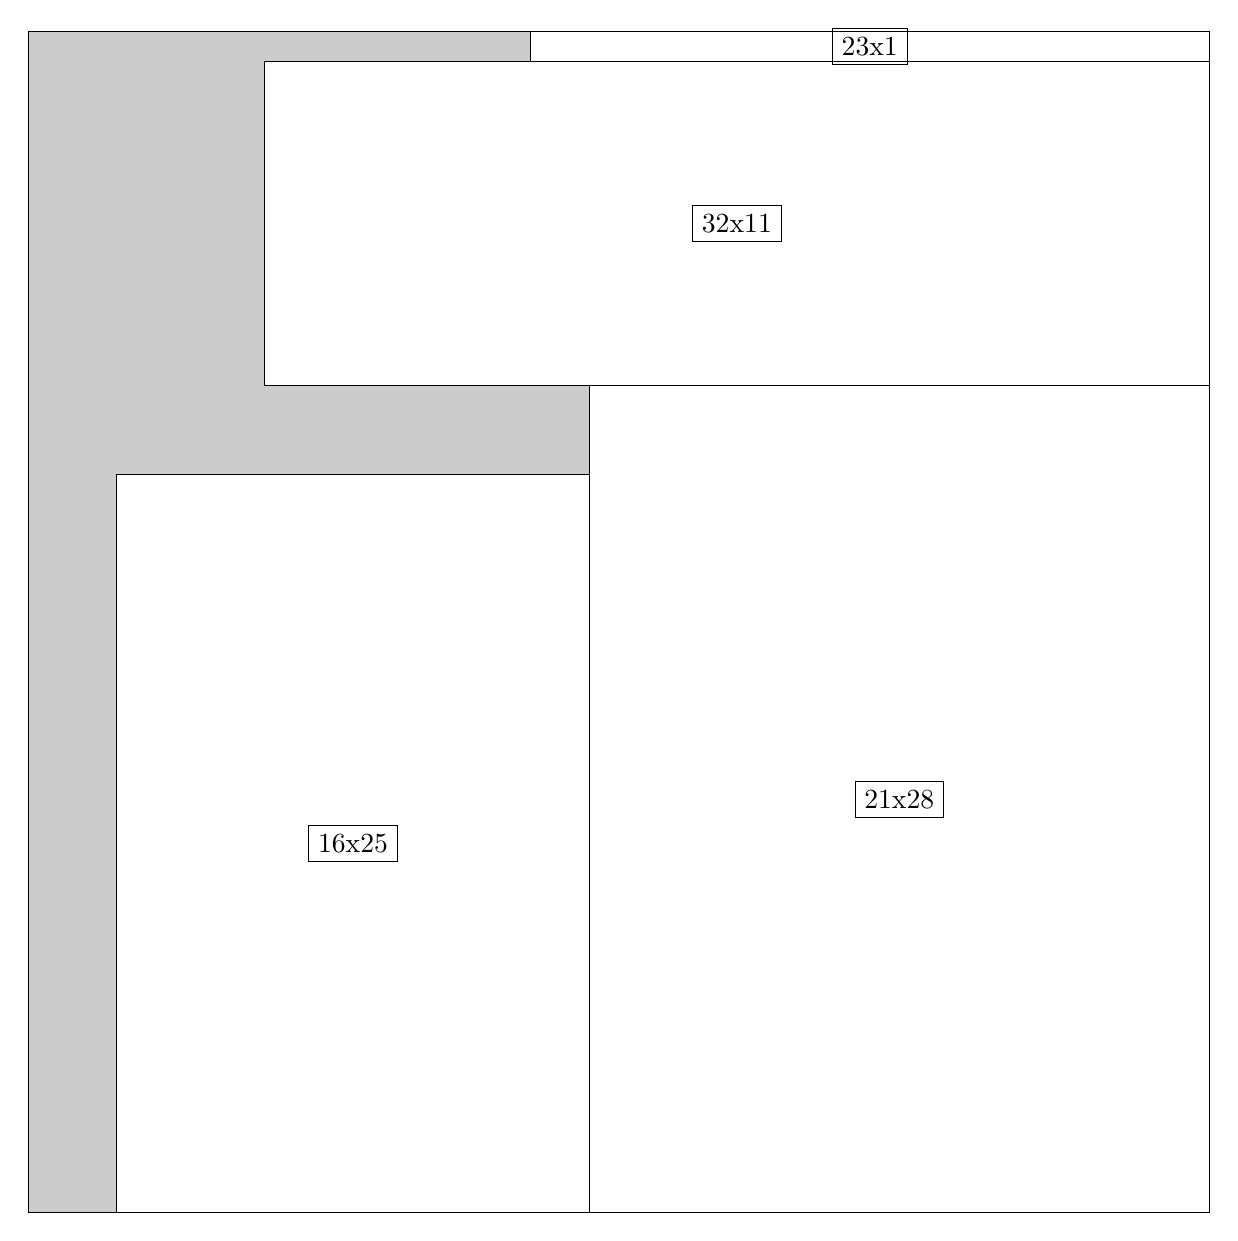
\begin{tikzpicture}[shorten >=1pt,scale=1.0,every node/.style={scale=1.0},->]
\tikzstyle{vertex}=[circle,fill=black!25,minimum size=14pt,inner sep=0pt]
\filldraw[fill=gray!40!white, draw=black] (0,0) rectangle (15.0,15.0);
\foreach \name/\x/\y/\w/\h in {21x28/7.125/0.0/7.875/10.5,16x25/1.125/0.0/6.0/9.375,32x11/3.0/10.5/12.0/4.125,23x1/6.375/14.625/8.625/0.375}
\filldraw[fill=white!40!white, draw=black] (\x,\y) rectangle node[draw] (\name) {\name} ++(\w,\h);
\end{tikzpicture}


w =21 , h =28 , x =19 , y =0 , v =588
\par
w =16 , h =25 , x =3 , y =0 , v =400
\par
w =32 , h =11 , x =8 , y =28 , v =352
\par
w =23 , h =1 , x =17 , y =39 , v =23
\par
\newpage


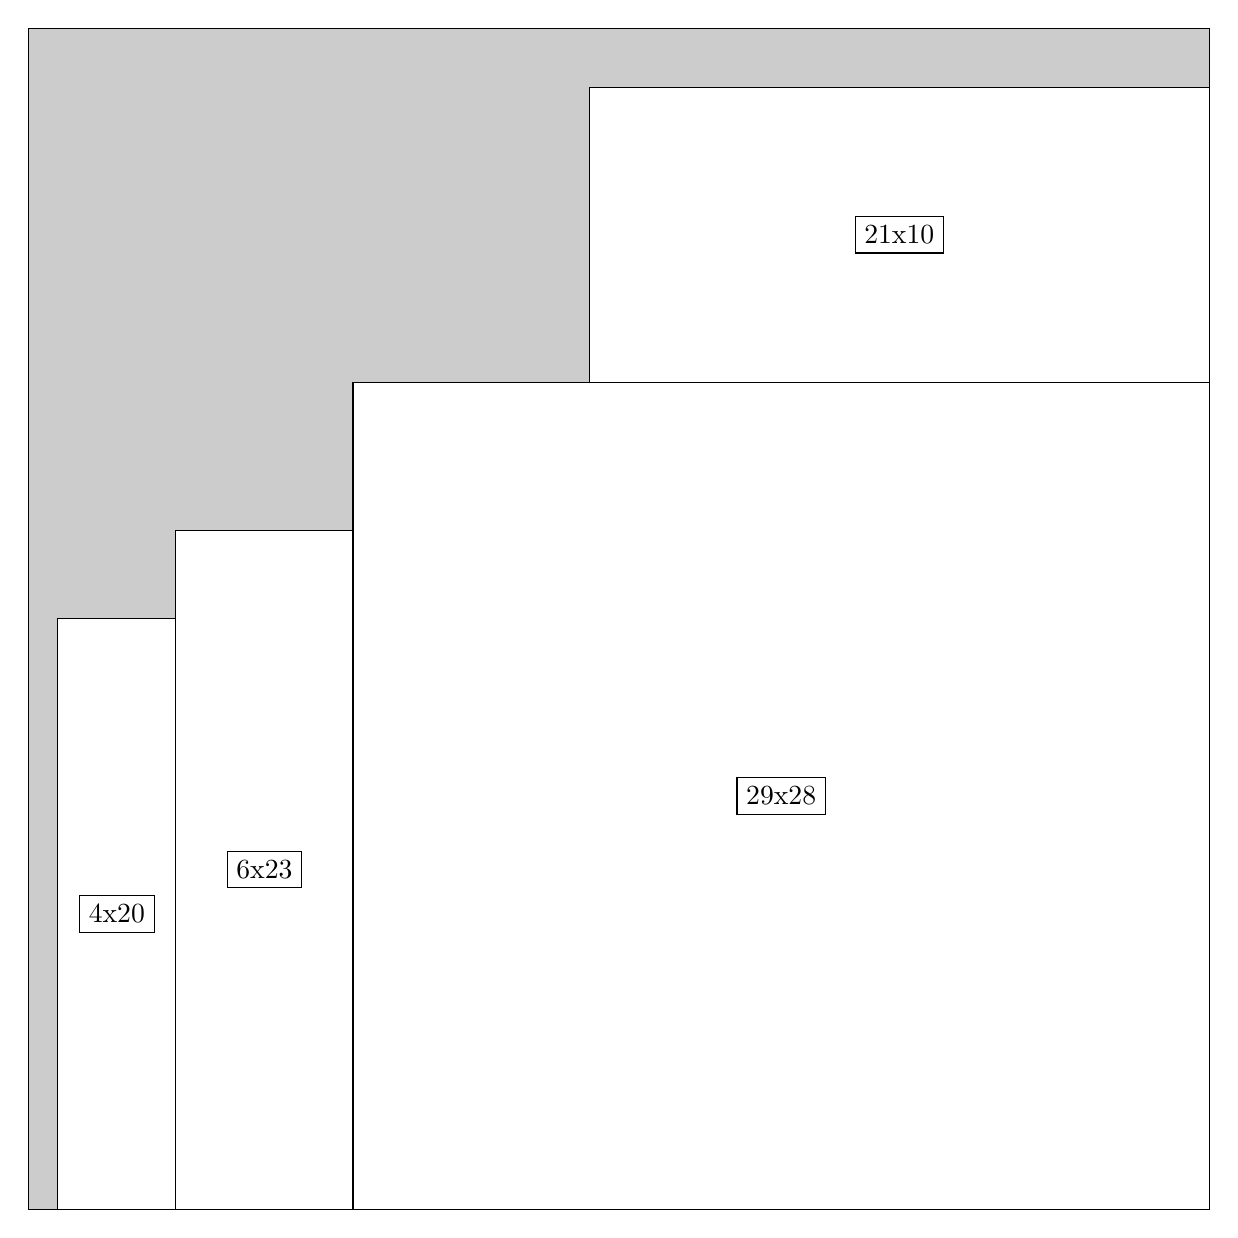
\begin{tikzpicture}[shorten >=1pt,scale=1.0,every node/.style={scale=1.0},->]
\tikzstyle{vertex}=[circle,fill=black!25,minimum size=14pt,inner sep=0pt]
\filldraw[fill=gray!40!white, draw=black] (0,0) rectangle (15.0,15.0);
\foreach \name/\x/\y/\w/\h in {29x28/4.125/0.0/10.875/10.5,21x10/7.125/10.5/7.875/3.75,6x23/1.875/0.0/2.25/8.625,4x20/0.375/0.0/1.5/7.5}
\filldraw[fill=white!40!white, draw=black] (\x,\y) rectangle node[draw] (\name) {\name} ++(\w,\h);
\end{tikzpicture}


w =29 , h =28 , x =11 , y =0 , v =812
\par
w =21 , h =10 , x =19 , y =28 , v =210
\par
w =6 , h =23 , x =5 , y =0 , v =138
\par
w =4 , h =20 , x =1 , y =0 , v =80
\par
\newpage


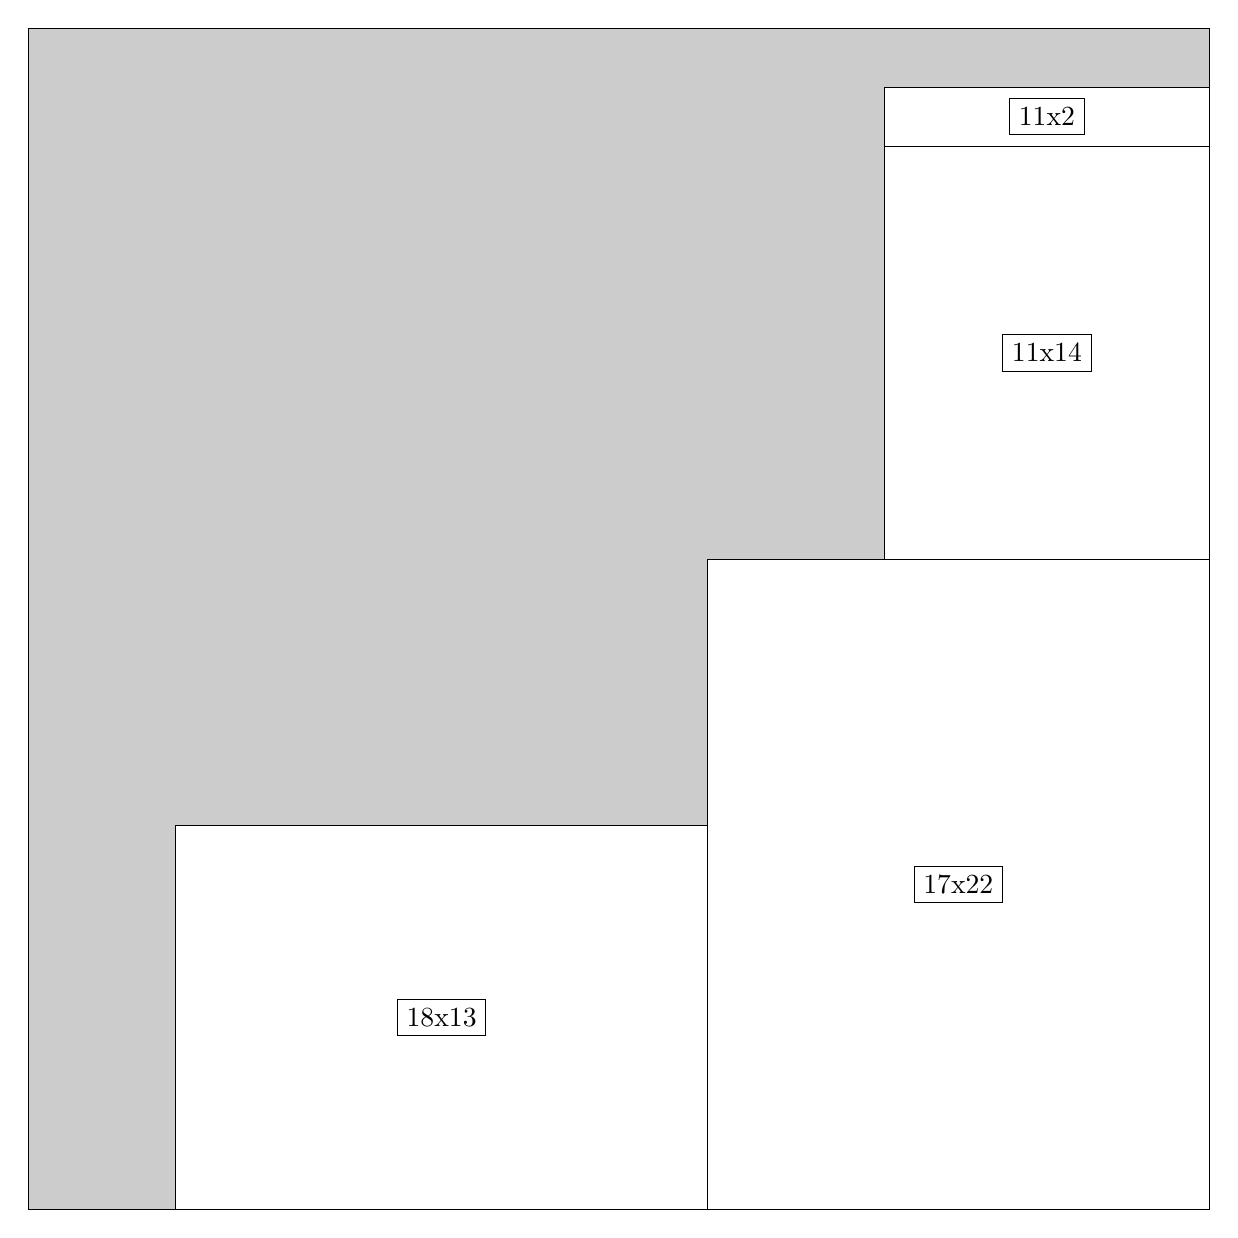
\begin{tikzpicture}[shorten >=1pt,scale=1.0,every node/.style={scale=1.0},->]
\tikzstyle{vertex}=[circle,fill=black!25,minimum size=14pt,inner sep=0pt]
\filldraw[fill=gray!40!white, draw=black] (0,0) rectangle (15.0,15.0);
\foreach \name/\x/\y/\w/\h in {17x22/8.625/0.0/6.375/8.25,11x14/10.875/8.25/4.125/5.25,11x2/10.875/13.5/4.125/0.75,18x13/1.875/0.0/6.75/4.875}
\filldraw[fill=white!40!white, draw=black] (\x,\y) rectangle node[draw] (\name) {\name} ++(\w,\h);
\end{tikzpicture}


w =17 , h =22 , x =23 , y =0 , v =374
\par
w =11 , h =14 , x =29 , y =22 , v =154
\par
w =11 , h =2 , x =29 , y =36 , v =22
\par
w =18 , h =13 , x =5 , y =0 , v =234
\par
\newpage


\end{document}